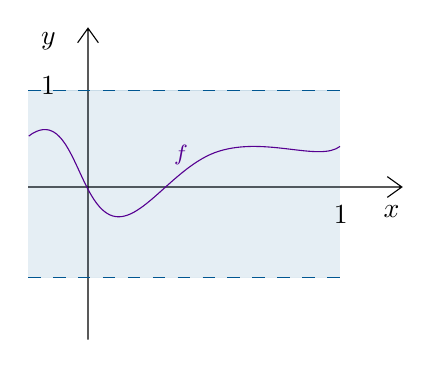
\begin{tikzpicture}[x=0.75pt,y=0.75pt,yscale=-1,xscale=1]
	%uncomment if require: \path (0,300); %set diagram left start at 0, and has height of 300

	%Shape: Axis 2D [id:dp0672040940975357] 
	\draw  (0,76.5) -- (180,76.5)(28.8,0) -- (28.8,150) (173,71.5) -- (180,76.5) -- (173,81.5) (23.8,7) -- (28.8,0) -- (33.8,7)  ;
	%Straight Lines [id:da19847713850781956] 
	\draw [color={rgb, 255:red, 0; green, 86; blue, 145 }  ,draw opacity=1 ][fill={rgb, 255:red, 0; green, 86; blue, 145 }  ,fill opacity=1 ] [dash pattern={on 4.5pt off 4.5pt}]  (0,120) -- (150,120) ;
	%Straight Lines [id:da26723242026257843] 
	\draw [color={rgb, 255:red, 0; green, 86; blue, 145 }  ,draw opacity=1 ][fill={rgb, 255:red, 0; green, 86; blue, 145 }  ,fill opacity=1 ] [dash pattern={on 4.5pt off 4.5pt}]  (0,30) -- (150,30) ;
	%Shape: Rectangle [id:dp7430552976593023] 
	\draw  [draw opacity=0][fill={rgb, 255:red, 0; green, 86; blue, 145 }  ,fill opacity=0.1 ] (0,30) -- (150,30) -- (150,120) -- (0,120) -- cycle ;
	%Curve Lines [id:da49050279449110856] 
	\draw [color={rgb, 255:red, 86; green, 0; blue, 145 }  ,draw opacity=1 ]   (0.23,51.95) .. controls (20.23,36.95) and (23.25,80.01) .. (38,89.21) .. controls (52.75,98.41) and (69.09,66.23) .. (92,59.21) .. controls (114.91,52.18) and (140.23,64.45) .. (150.23,56.95) ;

	% Text Node
	\draw (170,84) node [anchor=north west][inner sep=0.75pt]    {$x$};
	% Text Node
	\draw (5,1) node [anchor=north west][inner sep=0.75pt]    {$y$};
	% Text Node
	\draw (5,22) node [anchor=north west][inner sep=0.75pt]    {$1$};
	% Text Node
	\draw (69,55) node [anchor=north west][inner sep=0.75pt]  [font=\footnotesize,color={rgb, 255:red, 86; green, 0; blue, 145 }  ,opacity=1 ]  {$f$};
	% Text Node
	\draw (146,84) node [anchor=north west][inner sep=0.75pt]    {$1$};


\end{tikzpicture}
